\documentclass[8pt,draft]{beamer}
\usepackage{units,multicol,booktabs,tikz,xparse,tikz-3dplot,animate,mathtools}
\usepackage[labelformat=empty]{caption}
\usetikzlibrary{arrows.meta,calc,shapes,angles,quotes,patterns}

\graphicspath{{Images/}}

%Display framenumber in footer
\newcommand*\oldmacro{}%
\let\oldmacro\insertshorttitle%
\renewcommand*\insertshorttitle{%
  \oldmacro\hfill%
  \insertframenumber\,/\,\inserttotalframenumber}

%Choose colors for themes
\definecolor{myblue}{rgb}{0.2,0.2,0.7} %Default Warsaw
\definecolor{myred}{RGB}{165,8,8}
\definecolor{myviolet}{RGB}{100,8,165}
\definecolor{mygreen}{RGB}{0,132,15}

%Tikz colors
\definecolor{bluegrid}{RGB}{197,207,224}

% Initialize default color theme
\setbeamercolor{author in head/foot}{bg=black} 		%1501 foot
\setbeamercolor{subsection in head/foot}{bg=myblue} 	% lecture title foot
\setbeamercolor{section in head/foot}{bg=black} 		% frametitle gradient
\setbeamercolor{frametitle}{bg=myblue} 				%frametitle primary color
\setbeamercolor{local structure}{fg=black}				%Necessary for enumerate
\setbeamercolor{item projected}{bg=myblue}			%itemize bullets

% iClicker enumerate box drawing
\newcommand{\tikzmark}[1]{\tikz[overlay,remember picture] \node (#1) {};}

% Macros
\newcommand{\vect}[1]{\mathbf{#1}}
\newcommand{\vecth}[1]{\hat{\mathbf{#1}}}
\def\flb#1\fle{\begin{flalign*}#1\end{flalign*}} % begin / end full left align

% More Stuff
\usefonttheme[onlymath]{serif}
\setbeamercovered{invisible}
\hfuzz=60pt %Surpresses hbox full warnings by extending to 50pt
\newdimen\hfuzz
\vbadness = 10000 %Similar to hbox warning supression

% Mode
\mode<presentation>{\usetheme{Warsaw}}


% Generate Credentials
\title[Cosmological Fluctuations]{Cosmological Fluctuations in Standard and Conformal Gravity}
\author[Matthew Phelps]{Matthew Phelps}
\institute{\normalsize{Doctoral Degree Final Examination}
\and 
\includegraphics[width=0.8 in]{uconn-logo.png} }
\date{June 02, 2020}


%%%%%%%%%%%%%%%%%%%%%%%%%%%%%%%%%%%%%%%%%%%%%%%%%%%%%%%%%%%%%%
% Begin Document
%%%%%%%%%%%%%%%%%%%%%%%%%%%%%%%%%%%%%%%%%%%%%%%%%%%%%%%%%%%%%%
%\includeonlyframes{current}
\begin{document}
\beamertemplatenavigationsymbolsempty %Remove navigation icons
\setbeamertemplate{enumerate item}{(\Alph{enumi})} %Set default enumeration style


%%%%%%%%%%%%%%%%%%%%%%%%%%%%%%%%%%%%%%%%%%%%%%%%%%%%%%%%%%%%%%
% Slide  - Title Page
%%%%%%%%%%%%%%%%%%%%%%%%%%%%%%%%%%%%%%%%%%%%%%%%%%%%%%%%%%%%%%

\begingroup
\Large
\begin{frame}
\setcounter{framenumber}{0}
	\titlepage
\end{frame}
\endgroup

%%%%%%%%%%%%%%%%%%%%%%%%%%%%%%%%%%%%%%%%%%%%%%%%%%%%%%%%%%%%%%
% Slide  - TOC
%%%%%%%%%%%%%%%%%%%%%%%%%%%%%%%%%%%%%%%%%%%%%%%%%%%%%%%%%%%%%%

\begingroup
\Large
\begin{frame}{Overview}
	\begin{itemize}
		\item Introduction and Formalism
		\item Three Dimensional Scalar, Vector, Tensor Decomposition (SVT3)
		\item Four Dimensional Scalar, Vector, Tensor Decomposition (SVT4)
		\item Conformal Gravity (SVT and Conformal to Flat Backgrounds)
		\item Conformal Gravity Robertson-Walker Radiation Era Solution
		\item Computational Methods
		\item Conclusions
	\end{itemize}
\end{frame}
\endgroup

%%%%%%%%%%%%%%%%%%%%%%%%%%%%%%%%%%%%%%%%%%%%%%%%%%%%%%%%%%%%%%
% Slide  - Introduction and Formalism
%%%%%%%%%%%%%%%%%%%%%%%%%%%%%%%%%%%%%%%%%%%%%%%%%%%%%%%%%%%%%%

\begingroup
\Large
\begin{frame}{Introduction and Formalism Overview}
	\begin{itemize}
		\item Introduction and Formalism
		\begin{itemize}
			\large{
			\item Cosmological Geometries
			\item Einstein Gravity
			\item Perturbation Theory
			\item Gauge Transformations
			\item Solution Methods
			}
		\end{itemize}
	\end{itemize}
\end{frame}
\endgroup

%%%%%%%%%%%%%%%%%%%%%%%%%%%%%%%%%%%%%%%%%%%%%%%%%%%%%%%%%%%%%%
% Slide  - Cosmological Geometries 
%%%%%%%%%%%%%%%%%%%%%%%%%%%%%%%%%%%%%%%%%%%%%%%%%%%%%%%%%%%%%%

\begin{frame}{Cosmological Geometries}
	\begin{columns}
	\begin{column}{0.5\linewidth}
	\begin{itemize}
		\item Cosmological Principle: Structure of spacetime is homoegenous and isotropic at large scales
		\item Geometries: Robertson Walker (flat, spherical, hyperbolic), de Sitter ($dS_4 \subset \rm{RW}$)
		\item All background geometries relevant to cosmology can be expressed as conformal to flat
	\end{itemize}
	\begin{eqnarray*}
		ds^2 = \Omega(x)^2\big(-dt^2 + dx^2 + dy^2 + dz^2\big)
	\end{eqnarray*}
	\end{column}
	\begin{column}{0.5\linewidth}
		\begin{figure}
			\includegraphics[width=\linewidth]{hubble_deep.jpg}
			{\caption*{Hubble Ultra-Deep Field. NASA and the European Space Agency.}}
		\end{figure}
	\end{column}
	\end{columns}
\end{frame}

%%%%%%%%%%%%%%%%%%%%%%%%%%%%%%%%%%%%%%%%%%%%%%%%%%%%%%%%%%%%%%
% Slide  - Cosmological Geometries R.W. k=0
%%%%%%%%%%%%%%%%%%%%%%%%%%%%%%%%%%%%%%%%%%%%%%%%%%%%%%%%%%%%%%

\begin{frame}{Cosmological Geometries R.W.}
	Comoving Robertson Walker geometry:
	\begin{eqnarray*}
	ds^2 &=& -dt^2 + a(t)^2 \tilde g_{ij}dx^i dx^j
	\nonumber\\
	&=& -dt^2 + a(t)^2\bigg[\frac{dr^2}{1-kr^2} + r^2 d\theta^2 + r^2 \sin^2\theta d\phi^2\bigg]
	\end{eqnarray*}
	3-Space Curvature Tensors,
	\begin{eqnarray*}
	R_{ijkl} = k(\tilde g_{jk}\tilde g_{il} - \tilde g_{ik}\tilde g_{jl}), \qquad R_{ij} = -3k\tilde g_{ij}, \qquad R = -6k
	\end{eqnarray*}
	with $k \in \{-1,0,1\}$. Define the conformal time
	\begin{eqnarray*}
		\tau = \int \frac{dt}{a(t)},
	\end{eqnarray*}
	\only<1>{
	\begin{eqnarray*}
		ds^2 = a(\tau)^2\bigg[-d\tau^2 + \frac{dr^2}{1-kr^2} + r^2 d\theta^2 + r^2 \sin^2\theta d\phi^2\bigg]
	\end{eqnarray*}
	}
	\only<2>{
	set $k=0$ (flat), simple conformal to flat form
	\begin{eqnarray*}
		\boxed{ds^2 = a(\tau)^2\bigg[-d\tau^2 + dr^2 + r^2 d\theta^2 + r^2 \sin^2\theta d\phi^2\bigg]}
	\end{eqnarray*}		
	}
\end{frame}

%%%%%%%%%%%%%%%%%%%%%%%%%%%%%%%%%%%%%%%%%%%%%%%%%%%%%%%%%%%%%%
% Slide  - Cosmological Geometries R.W. k=1
%%%%%%%%%%%%%%%%%%%%%%%%%%%%%%%%%%%%%%%%%%%%%%%%%%%%%%%%%%%%%%

\begin{frame}{Cosmological Geometries R.W. $k=1$}
	$k=1$ (spherical)
	\begin{eqnarray*}
		ds^2 = a(\tau)^2\bigg[-d\tau^2 + \frac{dr^2}{1-r^2} + r^2 d\theta^2 + r^2 \sin^2\theta d\phi^2\bigg]
	\end{eqnarray*}	
	Set $\sin\chi = r$, $p = \tau$, 
	\begin{eqnarray*}
		ds^2 = a(p)^2\bigg[-dp^2 + d\chi^2 + \sin^2\chi d\theta^2 + \sin^2\chi \sin^2\theta d\phi^2\bigg]
	\end{eqnarray*}
	Introduce coordinates
	\begin{eqnarray*}
			p' + r' &=& \tan[(p+\chi)/2],\quad p'-r'=\tan[(p-\chi)/2]
			\nonumber\\
			p' &=& \frac{\sin p}{\cos p + \cos \chi}, \quad r' = \frac{\sin\chi}{\cos p + \cos\chi}
	\end{eqnarray*}
	\begin{eqnarray*}
	\implies \boxed{ds^2 = \frac{4a^2(p)}{[1+(p'+r')^2][1+(p'-r')^2]}[-dp'^2 + dr'^2 +r'^2 d\theta^2 + r'^2\sin^2\theta d\phi^2]}
	\end{eqnarray*}
\end{frame}

%%%%%%%%%%%%%%%%%%%%%%%%%%%%%%%%%%%%%%%%%%%%%%%%%%%%%%%%%%%%%%
% Slide  - Cosmological Geometries R.W. k=-1
%%%%%%%%%%%%%%%%%%%%%%%%%%%%%%%%%%%%%%%%%%%%%%%%%%%%%%%%%%%%%%

\begin{frame}{Cosmological Geometries R.W. $k=-1$}
	$k=-1$ (hyperbolic)
	\begin{eqnarray*}
		ds^2 = a(\tau)^2\bigg[-d\tau^2 + \frac{dr^2}{1+r^2}  + r^2 d\theta^2 + r^2 \sin^2\theta d\phi^2\bigg]
	\end{eqnarray*}	
	Set $\sinh\chi = r$, $p = \tau$, 
	\begin{eqnarray*}
		ds^2 = a(p)^2\bigg[-dp^2 + d\chi^2 + \sinh^2\chi d\theta^2 + \sinh^2\chi \sin^2\theta d\phi^2\bigg]
	\end{eqnarray*}
	Introduce coordinates
	\begin{eqnarray*}
		p' + r' &=& \tanh[(p+\chi)/2],\quad p'-r'=\tanh[(p-\chi)/2]
		\nonumber\\
		p' &=& \frac{\sinh p}{\cosh p + \cosh \chi}, \quad r' = \frac{\sinh\chi}{\cosh p + \cosh\chi}
	\end{eqnarray*}
	\begin{eqnarray*}
	\implies \boxed{ds^2 = \frac{4a^2(p)}{[1-(p'+r')^2][1-(p'-r')^2]}[-dp'^2 + dr'^2 +r'^2 d\theta^2 + r'^2\sin^2\theta d\phi^2]}
	\end{eqnarray*}
\end{frame}

%%%%%%%%%%%%%%%%%%%%%%%%%%%%%%%%%%%%%%%%%%%%%%%%%%%%%%%%%%%%%%
% Slide  - Einstein Gravity
%%%%%%%%%%%%%%%%%%%%%%%%%%%%%%%%%%%%%%%%%%%%%%%%%%%%%%%%%%%%%%

\begin{frame}{Einstein Gravity}
	Einstein Hilbert action
	\begin{eqnarray*}
	I_{\text{EH}} = -\frac{1}{16\pi G} \int d^4x (-g)^{1/2}  g^{\mu\nu}R_{\mu\nu}.
	\end{eqnarray*}
	Functional variation w.r.t $g_{\mu\nu}$ yields Einstein tensor,
	\begin{eqnarray*}
	\frac{16\pi G}{(-g)^{1/2}} \frac{\delta I_{\text{EH}}}{\delta g_{\mu\nu}}= G^{\mu\nu} = R^{\mu\nu} - \frac{1}{2}g^{\mu\nu}R^\alpha{}_\alpha,
	\end{eqnarray*}
	likewise, variation of matter action $I_{\rm M}$ w.r.t $g_{\mu\nu}$ yields Energy Momentum tensor
	\begin{eqnarray*}
	\frac{2}{(-g)^{1/2}} \frac{ \delta I_\text{M}}{\delta g_{\mu\nu}} = T_{\mu\nu}. 
	\end{eqnarray*}
	Requiring sum of actions to be stationary gives us Einstein field equations
	\begin{eqnarray*}
	R^{\mu\nu} - \frac{1}{2}g^{\mu\nu}R^\alpha{}_\alpha = -8\pi G T^{\mu\nu},
	\label{EinEOM}
	\end{eqnarray*}
	subject to Bianchi identity
	\begin{eqnarray*}
	\nabla_\mu R^{\mu\nu} = \frac{1}{2}\nabla^\nu R^\mu{}_\mu \implies \nabla_\mu G^{\mu\nu} = 0.
	\end{eqnarray*}
\end{frame}

%%%%%%%%%%%%%%%%%%%%%%%%%%%%%%%%%%%%%%%%%%%%%%%%%%%%%%%%%%%%%%
% Slide  - Perturbation Theory
%%%%%%%%%%%%%%%%%%%%%%%%%%%%%%%%%%%%%%%%%%%%%%%%%%%%%%%%%%%%%%

\begin{frame}{Cosmological Perturbation Theory}
	Decompose metric into background and fluctuation, truncating at linear order
	\begin{columns}
		\begin{column}{0.7\linewidth}
			\begin{eqnarray*}
				g_{\mu\nu}(x) &=& g_{\mu\nu}^{(0)}(x) + h_{\mu\nu}(x),\qquad g^{\mu\nu}_{(0)}h_{\mu\nu} \equiv h
				\\ \\
				G_{\mu\nu} &=& G_{\mu\nu}(g_{\mu\nu}^{(0)}) + \delta G_{\mu\nu}(h_{\mu\nu})
				\\ \\
				G_{\mu\nu}^{(0)} &=& R_{\mu\nu}^{(0)} -\frac{1}{2} g_{\mu\nu}^{(0)} R_\alpha^{(0)\alpha}
				\label{Einzero}
				\\ \\
				\delta G_{\mu\nu} &=& \delta R_{\mu\nu} - \frac{1}{2} h_{\mu\nu} R_\alpha^{(0)\alpha} -\frac{1}{2}g_{\mu\nu}\delta R^\alpha{}_\alpha.
			\end{eqnarray*}
			\hspace{.04\linewidth}Likewise perturb $T_{\mu\nu}$ around background
			\begin{eqnarray*}
				T_{\mu\nu} &=& T_{\mu\nu}(g_{\mu\nu}^{(0)}) + \delta T_{\mu\nu}(h_{\mu\nu})
			\end{eqnarray*}
		\end{column}
		\begin{column}{0.3\linewidth}
			\begin{figure}[t]
				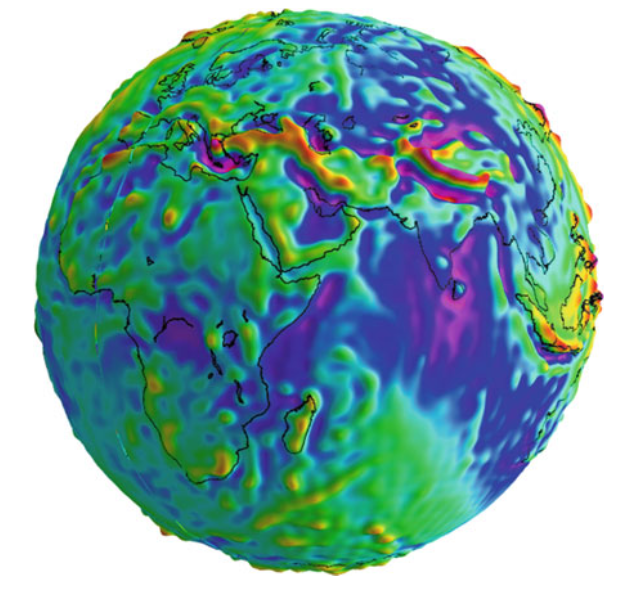
\includegraphics[width=\linewidth]{sphere_perturb.png}
			\end{figure}
			%\footnotemark
		\end{column}
	\end{columns}
	\vspace{1em}
	Form background and first order equations of motion (upon setting $8\pi G=1$)
	\begin{eqnarray*}
		\Delta_{\mu\nu}^{(0)} &=& G_{\mu\nu}^{(0)} + T_{\mu\nu}^{(0)} =0
		\\
		\Delta_{\mu\nu} &=& \delta G_{\mu\nu}^{(0)} + \delta T_{\mu\nu}^{(0)}=0
	\end{eqnarray*}
	\let\thefootnote\relax\footnotetext{Walter, U. (2019). Correction to: Astronautics. In Astronautics (pp. C1–C1). Springer International Publishing.}
\end{frame}

%%%%%%%%%%%%%%%%%%%%%%%%%%%%%%%%%%%%%%%%%%%%%%%%%%%%%%%%%%%%%%
% Slide  - Gauge Transformations
%%%%%%%%%%%%%%%%%%%%%%%%%%%%%%%%%%%%%%%%%%%%%%%%%%%%%%%%%%%%%%

\begin{frame}{Gauge Transformations}
	\begin{itemize}
		\item 	Under coordinate transformation $x^\mu \to x^\mu - \epsilon^\mu(x)$, with $\epsilon^\mu \sim \mathcal O(h)$, the perturbed metric transforms as
			\begin{eqnarray*}
				h_{\mu\nu} \to h_{\mu\nu} + \nabla_\mu \epsilon_\nu + \nabla_\nu \epsilon_\mu
			\end{eqnarray*}
		\item 	For every solution $h_{\mu\nu}$ to $\delta G_{\mu\nu} + \delta T_{\mu\nu} = 0$, a transformed $h'_{\mu\nu} = h_{\mu\nu} + \nabla_\mu \epsilon_\nu + \nabla_\nu \epsilon_\mu$ will also serve as a solution
		\item Set of four $\epsilon^\mu(x)$ define gauge freedom under coordinate transformation
		\item 10 components in $h_{\mu\nu}$, 4 coordinate transformations, leads to 6 independent degrees of freedom
		\item Under $x^\mu \to x^\mu - \epsilon^\mu(x)$, the perturbed tensors transform as
			\begin{eqnarray*}
				\delta G_{\mu\nu} \to \delta G_{\mu\nu} + {}^{(0)}G^\lambda{}_\mu \nabla_\nu \epsilon_\lambda +  {}^{(0)}G^{\lambda}{}_{\nu}\nabla_\mu \epsilon_\mu + \nabla_\lambda  G^{(0)}_{\mu\nu} \epsilon^\lambda
				\nonumber\\
				\delta T_{\mu\nu} \to \delta T_{\mu\nu} + {}^{(0)}T^\lambda{}_\mu \nabla_\nu \epsilon_\lambda +  {}^{(0)}T^{\lambda}{}_{\nu}\nabla_\mu \epsilon_\mu + \nabla_\lambda  T^{(0)}_{\mu\nu} \epsilon^\lambda.
			\end{eqnarray*}
		\item If background $G_{\mu\nu}^{(0)} = 0$ , then $\delta G_{\mu\nu}$ separately gauge invariant; likewise for vanishing background energy momentum tensor
		\item If $G_{\mu\nu}^{(0)} \ne 0$, then only the entire $\Delta_{\mu\nu} = \delta G_{\mu\nu} + T_{\mu\nu}$ is gauge invariant
	\end{itemize}


\end{frame}

%%%%%%%%%%%%%%%%%%%%%%%%%%%%%%%%%%%%%%%%%%%%%%%%%%%%%%%%%%%%%%
% Slide  - Solving Equations of Motion
%%%%%%%%%%%%%%%%%%%%%%%%%%%%%%%%%%%%%%%%%%%%%%%%%%%%%%%%%%%%%%

\begin{frame}{Solution Methods}
	\begin{itemize}
		\item Perturbed field equations $\delta G_{\mu\nu} + \delta T_{\mu\nu} = 0$ form a rather complex and extensive set of coupled tensor PDE's
		\item
		Much effort involved in simplifying, decoupling, and solving them
	\end{itemize}
	%
	\begin{eqnarray*}
		\delta G_{ij} &=& - \tfrac{1}{2} \overset{..}{h}_{ij} + \tfrac{1}{2} \overset{..}{h}_{00}{} \tilde{g}_{ij} + \tfrac{1}{2} \overset{..}{h} \tilde{g}_{ij} -  k \tilde{g}^{ba} \tilde{g}_{ij} h_{ab} + 3 k h_{ij} -  \dot{\Omega}^2 h_{ij} \Omega^{-2} -  \dot{\Omega}^2 \tilde{g}_{ij} h_{00}{} \Omega^{-2} 
		\nonumber\\
		&& -  \dot{h}_{ij} \dot{\Omega} \Omega^{-1}  + 2 \dot{h}_{00}{} \dot{\Omega} \tilde{g}_{ij} \Omega^{-1} + \dot{h} \dot{\Omega} \tilde{g}_{ij} \Omega^{-1} + 2 \overset{..}{\Omega} h_{ij} \Omega^{-1} + 2 \overset{..}{\Omega} \tilde{g}_{ij} h_{00}{} \Omega^{-1} 
		\nonumber\\
		&& + 2 \dot{\Omega} \tilde{g}^{ba} \tilde{g}_{ij} h_{0}{}_{b} \Omega^{-2} \tilde{\nabla}_{a}\Omega  - 2 \dot{h}_{0}{}_{b} \tilde{g}^{ba} \tilde{g}_{ij} \Omega^{-1} \tilde{\nabla}_{a}\Omega -  \tilde{g}^{ba} \tilde{g}_{ij} \tilde{\nabla}_{b}\dot{h}_{0}{}_{a} 
		\nonumber\\
		&& - 4 \tilde{g}^{ba} \tilde{g}_{ij} h_{0}{}_{a} \Omega^{-1} \tilde{\nabla}_{b}\dot{\Omega} + \tilde{g}^{ba} \Omega^{-1} \tilde{\nabla}_{a}\Omega \tilde{\nabla}_{b}h_{ij} - 2 \dot{\Omega} \tilde{g}^{ba} \tilde{g}_{ij} \Omega^{-1} \tilde{\nabla}_{b}h_{0}{}_{a}
		\nonumber\\
		&&  -  \tilde{g}^{ba} \tilde{g}_{ij} \Omega^{-1} \tilde{\nabla}_{a}h \tilde{\nabla}_{b}\Omega -  \tilde{g}^{ca} \tilde{g}^{db} \tilde{g}_{ij} h_{cd} \Omega^{-2} \tilde{\nabla}_{a}\Omega \tilde{\nabla}_{b}\Omega  + \tilde{g}^{ba} h_{ij} \Omega^{-2} \tilde{\nabla}_{a}\Omega \tilde{\nabla}_{b}\Omega 
		\nonumber\\
		&&+ \tfrac{1}{2} \tilde{g}^{ba} \tilde{\nabla}_{b}\tilde{\nabla}_{a}h_{ij} -  \tfrac{1}{2} \tilde{g}^{ba} \tilde{g}_{ij} \tilde{\nabla}_{b}\tilde{\nabla}_{a}h - 2 \tilde{g}^{ba} h_{ij} \Omega^{-1} \tilde{\nabla}_{b}\tilde{\nabla}_{a}\Omega  
		\nonumber\\
		&& -  \tfrac{1}{2} \tilde{g}^{ba} \tilde{\nabla}_{b}\tilde{\nabla}_{i}h_{ja} -  \tfrac{1}{2} \tilde{g}^{ba} \tilde{\nabla}_{b}\tilde{\nabla}_{j}h_{ia} + 2 \tilde{g}^{ca} \tilde{g}^{db} \tilde{g}_{ij} \Omega^{-1} \tilde{\nabla}_{a}\Omega \tilde{\nabla}_{d}h_{cb} 
		\nonumber\\
		&& + \tfrac{1}{2} \tilde{g}^{ca} \tilde{g}^{db} \tilde{g}_{ij} \tilde{\nabla}_{d}\tilde{\nabla}_{c}h_{ab}  + 2 \tilde{g}^{ca} \tilde{g}^{db} \tilde{g}_{ij} h_{ab} \Omega^{-1} \tilde{\nabla}_{d}\tilde{\nabla}_{c}\Omega + \tfrac{1}{2} \tilde{\nabla}_{i}\dot{h}_{0}{}_{j} 
		\nonumber\\
		&& -  \tilde{g}^{ba} \Omega^{-1} \tilde{\nabla}_{a}\Omega \tilde{\nabla}_{i}h_{jb} + \dot{\Omega} \Omega^{-1} \tilde{\nabla}_{i}h_{0}{}_{j} + \tfrac{1}{2} \tilde{\nabla}_{j}\dot{h}_{0}{}_{i} -  \tilde{g}^{ba} \Omega^{-1} \tilde{\nabla}_{a}\Omega \tilde{\nabla}_{j}h_{ib}
		\nonumber\\
		&&  + \dot{\Omega} \Omega^{-1} \tilde{\nabla}_{j}h_{0}{}_{i} + \tfrac{1}{2} \tilde{\nabla}_{j}\tilde{\nabla}_{i}h,
	\end{eqnarray*}

\end{frame}

%%%%%%%%%%%%%%%%%%%%%%%%%%%%%%%%%%%%%%%%%%%%%%%%%%%%%%%%%%%%%%
% Slide  - SVT3 Overview
%%%%%%%%%%%%%%%%%%%%%%%%%%%%%%%%%%%%%%%%%%%%%%%%%%%%%%%%%%%%%%

\begingroup
\Large
\begin{frame}{SVT3 Overview}
	\begin{itemize}
		\item Three-dimensional Scalar, Vector, Tensor Basis (SVT3)
		\begin{itemize}
			\large{
				\item SVT3 Decomposition
				\item Decouple Einstein Fluctuations in a de Sitter Background
				\item Integral Formalism
			}
		\end{itemize}
	\end{itemize}
\end{frame}
\endgroup

%%%%%%%%%%%%%%%%%%%%%%%%%%%%%%%%%%%%%%%%%%%%%%%%%%%%%%%%%%%%%%
% Slide  - SVT3 Decomposition
%%%%%%%%%%%%%%%%%%%%%%%%%%%%%%%%%%%%%%%%%%%%%%%%%%%%%%%%%%%%%%

\begin{frame}{SVT3 Decomposition}
	Decompose the metric perturbation $h_{\mu\nu}$ into a set of scalars, vectors, and tensors according to their transformation behavior under 3D rotations
	\begin{itemize}
		\item Define $h_{\mu\nu} = \Omega^2(x)f_{\mu\nu}$, perform 3 + 1 decomposition
		\begin{eqnarray*}
			ds^2 &=& g_{\mu\nu}dx^\mu dx^\nu = (g_{\mu\nu}^{(0)} + h_{\mu\nu})dx^\mu dx^\nu
			\\
			&=& \Omega^2(x)(\tilde g_{\mu\nu}^{(0)} + f_{\mu\nu})dx^\mu dx^\nu
			\\
			&=& \Omega^2(x)\big[(-1+f_{00})dt^2 + 2f_{0i}dtdx^i + (\tilde g_{ij} + f_{ij})\big]dx^i dx^j
			\\
		\end{eqnarray*}
		\vspace{-8mm}
		\item Decompose $f_{00}$, $f_{0i}$, and $f_{ij}$ in terms of 3-dimensional scalars, vectors, and tensors
		\begin{eqnarray*}
			f_{00} &=& -2\phi,\qquad f_{0i} = B_i + \tilde\nabla_i B
			\\
			f_{ij} &=& -2\psi \tilde g_{ij} + 2\tilde\nabla_i \tilde\nabla_j E + \tilde\nabla_i E_j + \tilde\nabla_j E_i + 2E_{ij},
		\end{eqnarray*}
		with vectors and tensors obeying
		\begin{eqnarray*}
			\tilde\nabla^i B_i = \tilde\nabla^i E_i = 0,\quad E_{ij} = E_{ji},\quad\tilde\nabla^i E_{ij} = 0,\quad \delta^{ij}E_{ij} = 0.
		\end{eqnarray*}
		\begin{eqnarray*}
			ds^2 &=& \Omega^2(x)\bigg[-(1+2\phi)dt^2 + 2(B_i + \tilde\nabla_i B)dt dx^i 
			\\&&+ [(1-2\psi)\tilde g_{ij} + 2\tilde\nabla_i \tilde\nabla_j E + \tilde\nabla_i E_j + \tilde\nabla_j E_i + 2E_{ij}]dx^i dx^j\bigg],
		\end{eqnarray*}
	\end{itemize}
\end{frame}

%%%%%%%%%%%%%%%%%%%%%%%%%%%%%%%%%%%%%%%%%%%%%%%%%%%%%%%%%%%%%%
% Slide  - SVT3 $\delta G_{\mu\nu}$ de Sitter 1/4
%%%%%%%%%%%%%%%%%%%%%%%%%%%%%%%%%%%%%%%%%%%%%%%%%%%%%%%%%%%%%%

\begin{frame}{SVT3 $\delta G_{\mu\nu}$ in a de Sitter Background}
	\begin{itemize}
		\only<1>{\item de Sitter geometry
				\begin{eqnarray*}
			ds^2 &=&\frac{1}{H^2\tau^2}\bigg[-(1+2\phi)dt^2 + 2(B_i + \tilde\nabla_i B)dt dx^i 
			\\&&+ [(1-2\psi)\delta_{ij} + 2\tilde\nabla_i \tilde\nabla_j E + \tilde\nabla_i E_j + \tilde\nabla_j E_i + 2E_{ij}]dx^i dx^j\bigg],
		\end{eqnarray*}
		}
		\item Energy momentum tensor
			\begin{eqnarray*}
				T_{\mu\nu} = -3H^2g_{\mu\nu} \implies \delta T_{\mu\nu} = -3 H^2 h_{\mu\nu} =-3H^2\Omega(\tau)^2f_{\mu\nu} 
			\end{eqnarray*}
		\item Insert the SVT3 decomposed $h_{\mu\nu}$ into a 3+1 $\delta G_{\mu\nu}$
	\end{itemize}
	\only<2->{
	\begin{eqnarray*}
	\delta G_{00}&=&-\frac{6}{\tau}\dot{\psi}-\frac{2}{\tau}\tilde{\nabla}^2(\tau \psi +B-\dot{E}),
	\nonumber\\
	\delta G_{0i}&=&\frac{1}{2}\tilde{\nabla}^2(B_i-\dot{E}_i)+\frac{1}{\tau^2}\tilde{\nabla}_i(3B-2\tau^2\dot{\psi}+2\tau \phi)+\frac{3}{\tau^2}B_i,
	\nonumber\\
	\delta G_{ij}&=&\frac{\delta_{ij}}{\tau^2}\bigg[-2\tau^2\ddot{\psi}+2\tau\dot{\phi}+4\tau\dot{\psi}-6\phi-6\psi
	\nonumber\\
	&+&\tilde{\nabla}^2\left(2\tau B-\tau^2\dot{B}+\tau^2\ddot{E}-2\tau\dot{E}-\tau^2\phi+\tau^2\psi\right)\bigg]
	\nonumber\\
	&+&\frac{1}{\tau^2}\tilde{\nabla}_i\tilde{\nabla}_j\left[-2\tau B +\tau^2\dot{B}-\tau^2\ddot{E}+2\tau\dot{E}+6E+\tau^2\phi-\tau^2\psi\right]
	\nonumber\\
	&+&\frac{1}{2\tau^2}\tilde{\nabla}_i\left[-2\tau B_j+2\tau\dot{E}_j+\tau^2\dot{B}_j-\tau^2\ddot{E}_j+6E_j\right]
	\nonumber\\
	&+&\frac{1}{2\tau^2}\tilde{\nabla}_j\left[-2\tau B_i+2\tau\dot{E}_i+\tau^2\dot{B}_i-\tau^2\ddot{E}_i+6E_i\right]
	\nonumber\\
	&-&\ddot{E}_{ij}+\frac{6}{\tau^2}E_{ij}+\frac{2}{\tau}\dot{E}_{ij}+\tilde{\nabla}^2E_{ij},
	\label{7.2}
	\end{eqnarray*}
}
\end{frame}

%%%%%%%%%%%%%%%%%%%%%%%%%%%%%%%%%%%%%%%%%%%%%%%%%%%%%%%%%%%%%%
% Slide  - SVT3 $\delta G_{\mu\nu}$ de Sitter 2/4
%%%%%%%%%%%%%%%%%%%%%%%%%%%%%%%%%%%%%%%%%%%%%%%%%%%%%%%%%%%%%%

\begin{frame}{SVT3 $\delta G_{\mu\nu}$ in a de Sitter Background}
	\begin{itemize}
		\item Compose $\Delta_{\mu\nu} = \delta G_{\mu\nu} + \delta T_{\mu\nu}$
	\end{itemize}
	\begin{eqnarray*}
	\Delta_{00}&=&-\frac{6}{\tau^2}(\dot{\beta}-\alpha)-\frac{2}{\tau}\tilde{\nabla}^2\beta=0,
	\\
	\Delta_{0i}&=&\frac{1}{2}\tilde{\nabla}^2(B_i-\dot{E}_i)-\frac{2}{\tau}\tilde{\nabla}_i(\dot{\beta}-\alpha)=0,
	\\
	\Delta_{ij}&=&\frac{\delta_{ij}}{\tau^2}\left[-2\tau(\ddot{\beta}-\dot{\alpha})+6(\dot{\beta}-\alpha)+\tau \tilde{\nabla}^2(2\beta-\tau \alpha)\right]
	+\frac{1}{\tau}\tilde{\nabla}_i\tilde{\nabla}_j(-2 \beta +\tau\alpha)
	\\
	&+&\frac{1}{2\tau}\tilde{\nabla}_i[-2(B_j-\dot{E}_j)+\tau(\dot{B}_j-\ddot{E}_j)]
	+\frac{1}{2\tau}\tilde{\nabla}_j[-2(B_i-\dot{E}_i)+\tau(\dot{B}_i-\ddot{E}_i)]
	\\
	&-&\ddot{E}_{ij}+\frac{2}{\tau}\dot{E}_{ij}+\tilde{\nabla}^2E_{ij}=0,
	\\
	g^{\mu\nu}\Delta_{\mu\nu}&=&H^2[-6\tau(\ddot{\beta}-\dot{\alpha})+24(\dot{\beta}-\alpha)
	+6\tau \tilde{\nabla}^2\beta-2\tau^2\tilde{\nabla}^2\alpha]=0,
	\end{eqnarray*}
	\hspace{0.1\linewidth}where
	\begin{eqnarray*}
	\alpha=\phi+\psi+\dot{B}-\ddot{E} ,\quad \beta=\tau\psi+B-\dot{E}, \quad B_i-\dot{E}_i,\quad E_{ij}.
	\end{eqnarray*}
\end{frame}

%%%%%%%%%%%%%%%%%%%%%%%%%%%%%%%%%%%%%%%%%%%%%%%%%%%%%%%%%%%%%%
% Slide  - SVT3 $\delta G_{\mu\nu}$ de Sitter 3/4
%%%%%%%%%%%%%%%%%%%%%%%%%%%%%%%%%%%%%%%%%%%%%%%%%%%%%%%%%%%%%%

\begin{frame}{SVT3 $\delta G_{\mu\nu}$ in a de Sitter Background}
	\begin{itemize}
		\item Decouple scalar, vector, and tensor gauge invariants by applying higher derivatives
		\begin{eqnarray*}
		\tilde{\nabla}^4(\alpha+\dot{\beta})=0,\quad \tilde{\nabla}^4(\alpha-\dot{\beta})=0,
		\end{eqnarray*}
		\begin{eqnarray*}
		\tilde{\nabla}^4(B_i-\dot{E}_i)=0,
		\end{eqnarray*}
		\begin{eqnarray*}
		\tilde{\nabla}^4\left(-\ddot{E}_{ij}+\frac{2}{\tau}\dot{E}_{ij}+\tilde{\nabla}^2E_{ij}\right)=0.
		\end{eqnarray*}
		\item Recap:
		\begin{itemize}
			\item Perturb $\delta G_{\mu\nu}$ and $\delta T_{\mu\nu}$, evaluating in de Sitter background
			\item Decompose $h_{\mu\nu}$ into SVT3 components, inserting into fields equations
			\item Compose $\Delta_{\mu\nu} = \delta G_{\mu\nu} + \delta T_{\mu\nu} = 0$ to form evolution equations consisting entirely of gauge invariant quantities
			\item Apply higher derivatives to decouple SVT3 representations, solve
		\end{itemize}
	\end{itemize}
\end{frame}

%%%%%%%%%%%%%%%%%%%%%%%%%%%%%%%%%%%%%%%%%%%%%%%%%%%%%%%%%%%%%%
% Slide  - SVT3 Integral Formulation 1/3
%%%%%%%%%%%%%%%%%%%%%%%%%%%%%%%%%%%%%%%%%%%%%%%%%%%%%%%%%%%%%%

\begin{frame}{SVT3 Integral Formulation}
	\begin{itemize}
		\item How can we ensure such an SVT3 decomposition exists for the general $h_{\mu\nu}$? Let's recall
				\begin{eqnarray*}
			f_{00} &=& -2\phi,\qquad f_{0i} = B_i + \tilde\nabla_i B
			\\
			f_{ij} &=& -2\psi \tilde g_{ij} + 2\tilde\nabla_i \tilde\nabla_j E + \tilde\nabla_i E_j + \tilde\nabla_j E_i + 2E_{ij},
		\end{eqnarray*}
		\begin{eqnarray*}
			\tilde\nabla^i B_i = \tilde\nabla^i E_i = 0,\quad E_{ij} = E_{ji},\quad\tilde\nabla^i E_{ij} = 0,\quad \delta^{ij}E_{ij} = 0.
		\end{eqnarray*}
	\end{itemize}
\end{frame}

%%%%%%%%%%%%%%%%%%%%%%%%%%%%%%%%%%%%%%%%%%%%%%%%%%%%%%%%%%%%%%
% Slide  - SVT3 Integral Formulation 2/3
%%%%%%%%%%%%%%%%%%%%%%%%%%%%%%%%%%%%%%%%%%%%%%%%%%%%%%%%%%%%%%

\begin{frame}{SVT3 Integral Formulation}
	Decomposition of $A_i = A_i^T + \partial_i A^L$
	\begin{itemize}
		\item Green's Identity
		\begin{eqnarray*}
			adf
		\end{eqnarray*}
	\end{itemize}
\end{frame}

%%%%%%%%%%%%%%%%%%%%%%%%%%%%%%%%%%%%%%%%%%%%%%%%%%%%%%%%%%%%%%
% Slide  - Conformal Gravity
%%%%%%%%%%%%%%%%%%%%%%%%%%%%%%%%%%%%%%%%%%%%%%%%%%%%%%%%%%%%%%

\begin{frame}{Conformal Gravity Intro.}
	\begin{eqnarray*}
		I_\text{W} &=& -\alpha_g \int d^4x (-g)^{1/2}C_{\lambda\mu\nu\kappa}C^{\lambda\mu\nu\kappa}
		\nonumber\\
		&\equiv& -2\alpha_g \int d^4x(-g)^{1/2}\left[R_{\mu\nu}R^{\mu\nu} - \tfrac{1}{3}(R^\alpha{}_\alpha)^2\right],
		\label{IW}
	\end{eqnarray*}
	\begin{eqnarray*}
		C_{\lambda\mu\nu\kappa}&=& R_{\lambda\mu\nu\kappa}
		-\frac{1}{2}\left(g_{\lambda\nu}R_{\mu\kappa}-
		g_{\lambda\kappa}R_{\mu\nu}-
		g_{\mu\nu}R_{\lambda\kappa}+
		g_{\mu\kappa}R_{\lambda\nu}\right)
		\\
		&&+\frac{1}{6}R^{\alpha}_{\phantom{\alpha}\alpha}\left(
		g_{\lambda\nu}g_{\mu\kappa}-
		g_{\lambda\kappa}g_{\mu\nu}\right)
	\end{eqnarray*}
	\begin{eqnarray*}
		-\frac{2}{(-g)^{1/2}} \frac{\delta I_{\text{W}}}{\delta g_{\mu\nu}}= 4\alpha_gW^{\mu\nu} = 4\alpha_g \left[2\nabla_\kappa\nabla_\lambda C^{\mu\lambda\nu\kappa} - R_{\kappa\lambda}C^{\mu\lambda\nu\kappa}\right].
		\label{Bachtensor}
	\end{eqnarray*}
\end{frame}
%%%%%%%%%%%%%%%%%%%%%%%%%%%%%%%%%%%%%%%%%%%%%%%%%%%%%%%%%%%%%%
% Slide  - 
%%%%%%%%%%%%%%%%%%%%%%%%%%%%%%%%%%%%%%%%%%%%%%%%%%%%%%%%%%%%%%

\begin{frame}{}

\end{frame}
%%%%%%%%%%%%%%%%%%%%%%%%%%%%%%%%%%%%%%%%%%%%%%%%%%%%%%%%%%%%%%
% Slide  - 
%%%%%%%%%%%%%%%%%%%%%%%%%%%%%%%%%%%%%%%%%%%%%%%%%%%%%%%%%%%%%%

\begin{frame}{}
	
\end{frame}
%%%%%%%%%%%%%%%%%%%%%%%%%%%%%%%%%%%%%%%%%%%%%%%%%%%%%%%%%%%%%%
% Slide  - 
%%%%%%%%%%%%%%%%%%%%%%%%%%%%%%%%%%%%%%%%%%%%%%%%%%%%%%%%%%%%%%

\begin{frame}{}
	
\end{frame}
%%%%%%%%%%%%%%%%%%%%%%%%%%%%%%%%%%%%%%%%%%%%%%%%%%%%%%%%%%%%%%
% End Document
%%%%%%%%%%%%%%%%%%%%%%%%%%%%%%%%%%%%%%%%%%%%%%%%%%%%%%%%%%%%%%

\end{document}